%%%%%% CMB-S4 Simulations and Data Analysis Chapter, Forecasting Section  %%%%%%%%%%%%%%%%

\section{Forecasting}\label{sec:Forecasting}

Given the computational constraints on time-domain simulations and analyses, it is currently not possible to use the production pipeline to explore the full instrument and observation parameter space. However, such exploration is critical in the mission design and development phase, and so we employ a forecasting pipeline (Figure \ref{fig_fcast}) to bypass this bottleneck. This section outlines the forecasting methodology; specific results obtained from this appraoch are given in the preceeding science chapters.

\begin{figure}[htbp]
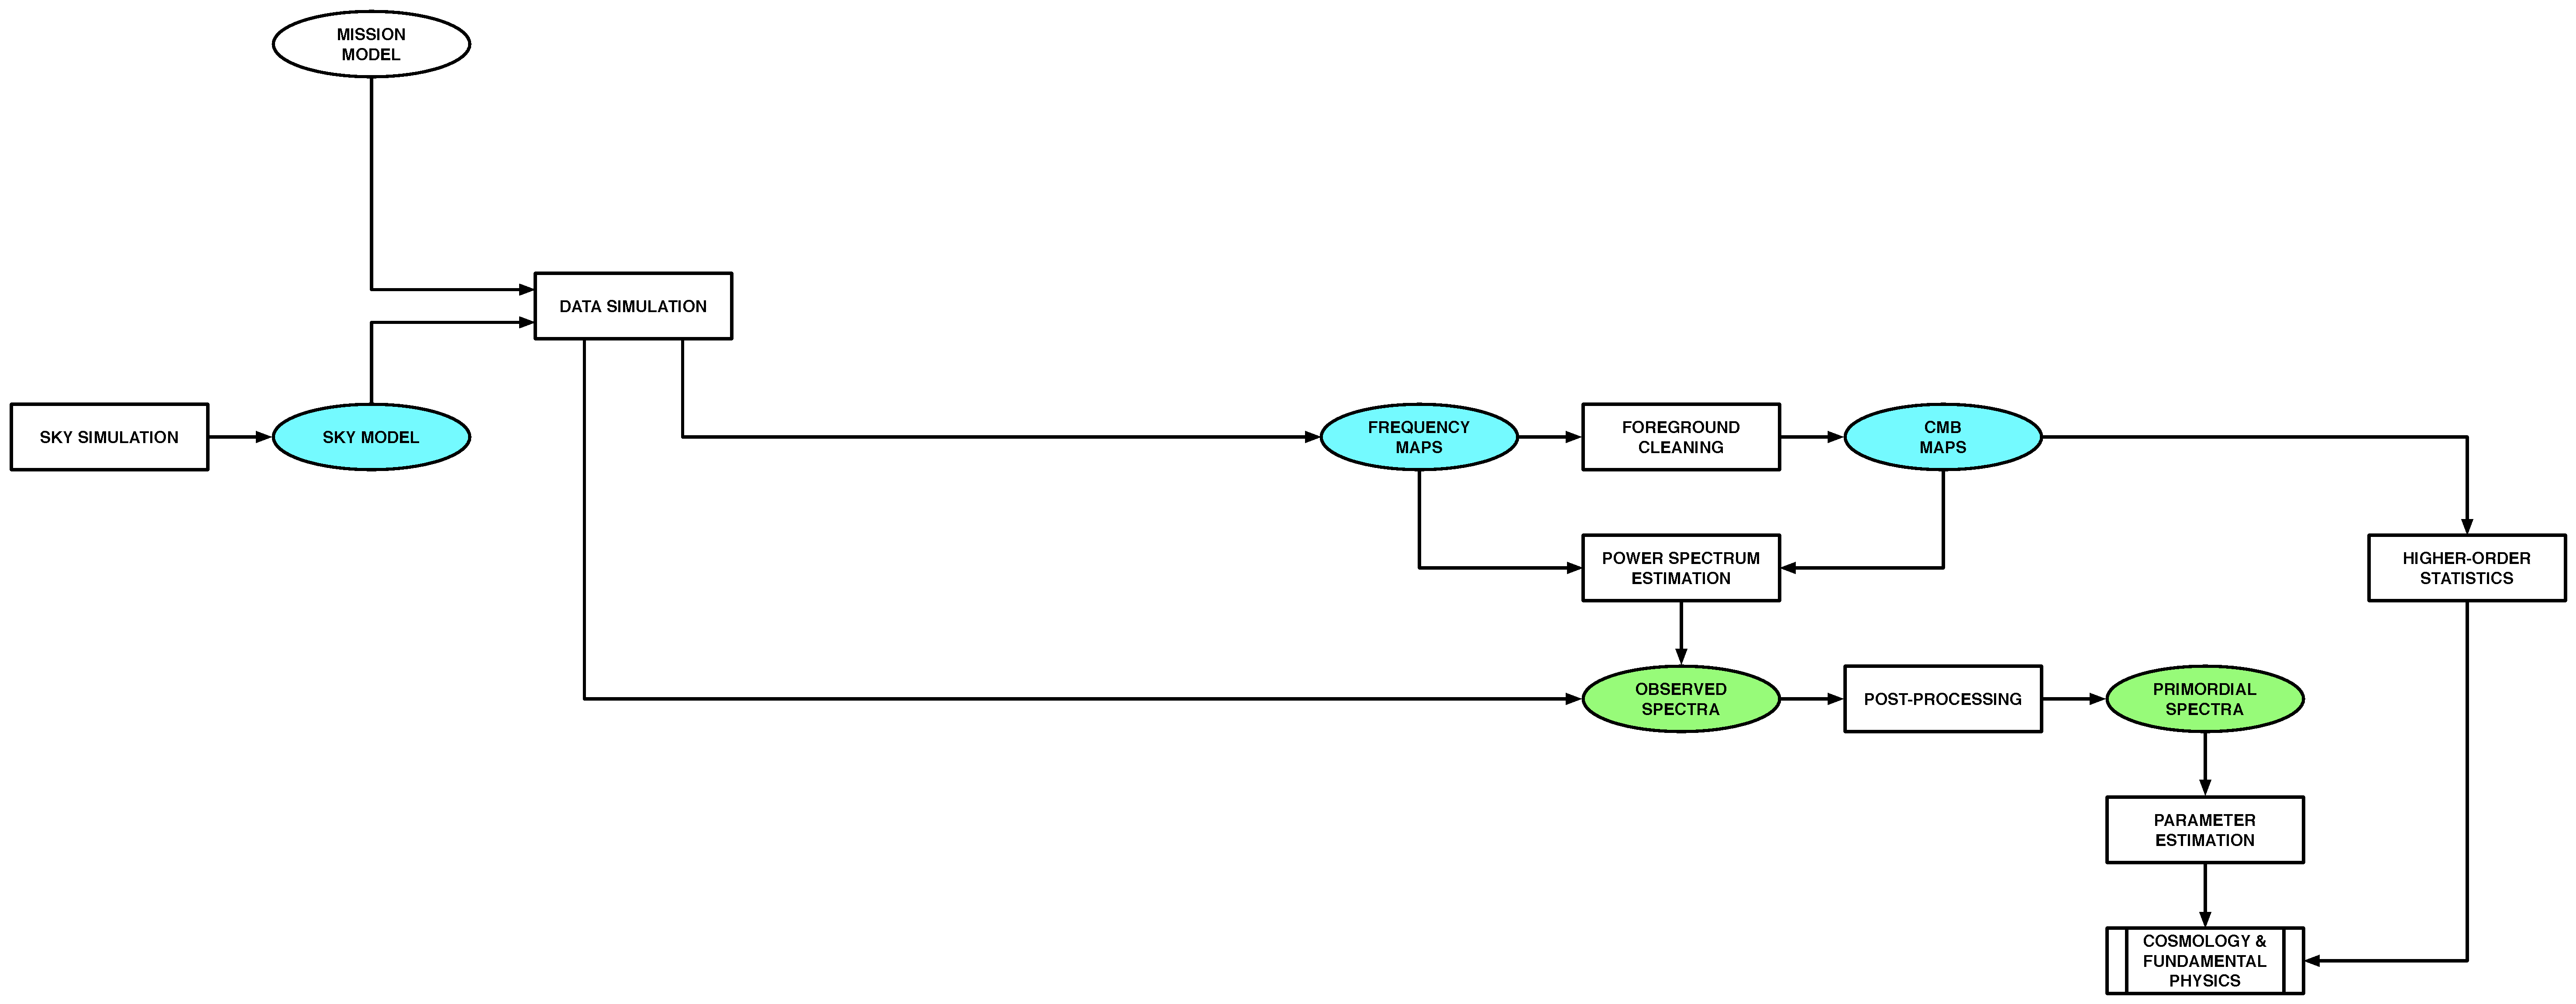
\includegraphics[width=0.9\textwidth]{Analysis/forecast}\\
\caption{The forecasting pipeline, including pixel- and spectral-domain simulations and analyses}
\label{fig_fcast}
\end{figure}

Forecasting efforts for Stage 1 and 2 experiments were hampered by lack of experience with previous deep polarization maps and little knowledge of high latitude Galactic foregrounds; forecasting for \cmbexp\ will therefore be built on the solid foundation of map-derived evaluations of instrumental noise performance and astrophysical foreground levels from the Stage 2 experiments and the Planck satellite.

The forecasting approach will combine Fisher matrix-derived estimates of power spectrum errors with detailed map-level simulations.
The spectral-domain projections are computationally easy, making them useful to explore the large parameter space of instrument and survey configurations.
Map-domain simulations are used to ground the spectral-domain projections in reality and to challenge them with cases of real world astrophysical complexity.
To gain the benefit of this complementarity, it is important that we maintain compatibility between these two forecasting approaches and establish agreement between them for simple questions before proceeding to more difficult tests.

A key input to the forecasting process are full-season noise maps from existing Stage 2 experiments, which encode actual noise performance and have been verified by null tests on real datasets.
Performance of \cmbexp\ can be estimated by rescaling these noise maps, which already contain reality factors such as detector yield, weather, observing efficiency, and filtering of sky modes.
Systematic errors should be included in the projections, with unknown systematics allowed at a level that scales with the map noise used for jackknife null tests.
Forecasting should also include our best knowledge of the astrophysical foregrounds and account for the impact of component separation on \cmbexp\ science goals.
The forecasting inputs will improve as we acquire data from Stage 3 experiments and possible complementary balloon-borne experiments, which will produce deeper noise maps and better assessments of foregrounds, as well as demonstrations of new techniques and technologies in development for Stage 4.

Here we describe the main approaches used by our community for forecasting the expected performance of \cmbexp. The central considerations for assessing the expected performance for large-scale B-modes are Galactic foregrounds, ability to delens the data, and a realistic assessment of instrument noise at large scales. 
For the smaller-scale polarization two-point functions (TE, EE) and the lensing four-point function ($\kappa \kappa$), extragalactic foregrounds and instrumental noise are the key considerations.
To forecast the return of the thermal Sunyaev-Zel'dovich effects, an estimate of the expected cluster counts as a function of mass and redshift is the core statistic, combined with an estimate of how well the masses can be calibrated using optical or CMB weak lensing. For the kinetic Sunyaev-Zeldovich effect, extragalactic foregrounds and overlap with spectroscopic surveys must all be considered. 

\subsection{Forecasting \cmbexp\ constraints on the tensor-to-scalar ratio}

\subsubsection{Spectrum-based domain forecasting}
\label{sec_specforecast}

Power spectra are the primary tool used for CMB analysis.
Forecasting the power spectrum uncertainty and resulting parameter constraints for \cmbexp\ is an efficient and powerful tool to explore trade-offs in experiment design.

The bandpower covariance matrix describes the raw sensitivity of all auto and cross-spectra obtained between maps of T, E, and/or B modes at multiple observing frequencies, as well as the signal and noise correlations that exist between these spectra.
This covariance matrix includes contributions from the sample variance of signal fields (CMB and foreground) and instrumental noise, including signal$\times$noise terms.
The signal variance depends on the assumed sky model, which can be modified to explore optimistic or pessimistic scenarios.
As discussed above, estimates of the noise variance should be obtained by rescaling of noise levels that have actually been obtained by Stage 2 experiments (or Stage 3, when available).
Only these scaled noise levels will include all the small ``reality factors'' that are incurred in operating a CMB experiment.

We will explicitly account for the impact of systematic errors by including them in the bandpower covariance matrix.
For constraining tensor-to-scalar ratio, we are particularly concerned with effects that add B-mode power to maps.
Even if the bandpowers are debiased using accurate simulations of such a systematic, it will still leave behind a noise floor due to its sample variance.
Unknown and unforseen sources of spurious signal in \cmbexp\ will ultimately be constrained by jackknife null tests, which analyze a map constructed from the difference of two data subsets.
The statistical power of the null test is set by the noise level of the maps, since any signal contributions should difference away.
We can acknowledge this limitation by including in our projections an unknown systematic that adds B modes at the level of the null test uncertainty.
Errors that are multiplicative in the signal, such as an absolute calibration error in the map, are best handled by adding nuisance parameters to the signal model.

Once we have a projection for the bandpower covariance matrix of \cmbexp\, we can derive constraints on a parametrized model of cosmological and foreground signals via the Fisher information matrix.
While we are most interested in parameter $r$, it is necessary to also consider the amplitude, spectrum, and spatial distribution of the dust and synchrotron foregrounds (see \cite{Ade:2015tva} for an example).
The Fisher matrix formalism allows us to calculate the marginalized error on each parameter, with priors if desired, or to explore the degeneracies between parameters.

By compressing the data down to power spectra, it is feasible to use this technique to evaluate a wide range of survey designs.
The parametrized signal model is also quite flexible and can include complications such as dust--synchrotron correlation or spatially varying foreground spectral indices.
The limitation is that by considering the power spectrum only we are treating all signals as Gaussian, an approximation which must break down at some point for foregrounds.
For this reason, it is important to have the ability to spot check the spectrum-based forecasts against map-based forecasts at specific choices of signal model.

As described in Section~\ref{sec:needs}, the specific implementation of Fisher forecasting for CMB-S4 constraints
on $r$ in this document assume the following baseline instrument configuration parameters:
%
\begin{itemize}
\item{250,000 detectors operating for four years, dedicated solely to the combination of measuring degree-scale B modes and measuring lensing B modes on the same patch of sky. The split in effort between degree-scale observations and lensing observations depends on the fraction of sky observed, which sets the level of delensing needed.}
\item{Eight frequency bands, two each in the four atmospheric windows between 30 and 300 GHz.}
\item{For the degree-scale effort, bandpower covariance matrices scaled directly from achieved BICEP2/Keck performance.}
\item{Foregrounds as measured in the BICEP2/Keck patch of sky, including decorrelation of the dust signal between high frequencies and the frequencies of interest for CMB.}
\item{Delensing efficiency based solely on noise level in the high-resolution map used for delensing---i.e., no degradation to delensing from foregrounds or systematics.}
\end{itemize}
%
In Section~\ref{sec:needs}, these assumptions are used to search sky fraction and detector effort parameter space, with 
$\sigma(r)$ as the figure of merit. We verify these results using a second Fisher code (described below) and a map-based
forecasting method (see next section).

The second Fisher code---detailed in \cite{Errard:2015cxa}---parameterizes the CMB-S4 instrument by its sky and multipole coverage, along with the central frequency, bandwidth, resolution and white-noise level of each channel. The ability of the instrument to remove diffuse foregrounds is estimated using a parametric maximum-likelihood forecast \cite{Errard:2011vi,Errard:2012qx} based on Planck foreground measurements \cite{Adam:2015tpy,Adam:2015wua}. The impacts of foreground subtraction---residual foregrounds and increased noise relative to the raw combination of all channels---are propagated to a delensing forecast (based on \cite{Smith:2010gu}), which also estimates the sensitivity to the lensing convergence power spectrum. Constraints on $r$ are produced with a standard Fisher forecast (see Section~\ref{sec:ttee} for a complete description) using temperature, $E$-mode, delensed-$B$-mode and lensing convergence information, marginalizing over the amplitude and multipole-dependence of the foreground residuals. As the mitigation of systematic effects is not currently modelled within this code, constraints on $r$ are typically a factor of 2.5 more optimistic than when these effects are included.

\subsubsection{Map-based domain forecasting}

Foregrounds are intrinsically non-Gaussian and anisotropic, so we also consider approaches directly in map space to explore the robustness of spectrum-based approaches, in particular in the case of pessimistic foregrounds where the spectral indices or dust emissivities have non-trivial spatial variation. The map-based method used in this Science Book is a Bayesian model fitting method, where the foregrounds are described parametrically using a physical model for each component. It is described in \cite{Alonso:prep} and follows similar implementations in e.g., \cite{Eriksen:2005dr}.

Using this method, we simulate maps of the CMB, Galactic foregrounds and expected noise at each of the \cmbexp\ frequencies and integrate them across the expected bandpass width for each channel. We use the PySM numerical code\footnote{\url{https://github.com/bthorne93/PySM}} which generates Galactic models as described for example in Section \ref{sec:skymodel}. Other similar codes exist in our community \cite{Delabrouille:2012ye}. In this framework it is straightforward to include simulations at ancillary frequencies that might be provided by other experiments, for example the Planck data. We fit a parameterized model to the simulated maps, fitting the CMB, thermal dust, and synchrotron in small pixels, and the synchrotron spectral index and dust emissivity and temperature in larger pixels of order degree-scale or larger. We estimate the BB power spectrum of the foreground-marginalized CMB map using the MASTER \cite{Hivon:2001jp} algorithm, and convert this into an estimate of $r$ and its uncertainty. In this Science Book we use the BFoRe code \cite{Alonso:prep}; our community also has access to the Commander code which can be used to perform similar analyses.

This method provides an assessment of the expected bias on $r$ if the model does not match the simulation, and shows how much the expected uncertainty on $r$ would increase if more complicated foreground models are explored e.g. \cite{ArmitageCaplan:2011sn,Remazeilles:2015hpa}. It is more computationally expensive than spectral-domain forecasts though, so we limit this approach to a smaller subset of explorations. 

We compare this map-based forecasting to the results of the spectrum-based Fisher-matrix 
forecasting described above. For discrete points in sky fraction and detector effort parameter space, 
we recover the Fisher results with the map-based code, both finding for example $\sigma(r)=0.001$ for $f_{\rm sky}=0.1$ and $r=0$. In this map-based approach we approximate the scaled achieved noise properties by modeling the noise as white noise plus a power-law noise component that starts dominating at a scale below $\ell_{\rm knee}$. The power law was determined by fitting to the achieved BICEP2/Keck noise surves.  This consistency of the different approaches indicates that foreground residuals due to assumptions of Gaussianity and isotropy are not significantly biasing the spctrum-based Fisher forecasts, but this will be the subject of further study as the S4 design evolves.

\subsection{Forecasting \cmbexp\ constraints on parameters from TT/TE/EE/$\kappa\kappa$}
\label{sec:ttee}

Throughout this Science Book we forecast the expected constraints on cosmological parameters from TT/TE/EE and $\kappa\kappa$ (the CMB lensing convergence power spectrum) using Fisher-matrix methods. This assumes that the resulting parameter distributions are close to Gaussian, which is sufficient for the majority of parameters we consider.

We assume that S4 data will be combined with existing Planck satellite data. We also assume that other non-CMB data will be available. In particular we consider measurements of Baryon Acoustic Oscillations from the DESI spectroscopic galaxy redshift survey. In some places we consider measurements of cosmic shear from the Large Synoptic Survey Telesope.


The codes we use either consider the unlensed maps and the lensing convergence map as the basic statistics, or the lensed power spectra of those maps together with the reconstructed $\kappa \kappa$ spectrum. For the power spectrum approach, to compute the Fisher matrix for the CMB we use the lensed power spectrum between each pair of fields $X, Y$:
%
\begin{equation}
\label{eqEstimator}
\hat{C}^{XY}_\ell = \frac{1}{2\ell+1}\sum_{m=-\ell}^{m=\ell} x^{*}_{\ell m} y_{\ell m}.
\end{equation}
%
The estimated power spectrum is Gaussian-distributed to good approximation at small scales. In this case a full-sky survey has
%
\begin{equation}
-2\ln\mathcal{L}(\boldsymbol{\theta}) = -2\sum_\ell \ln p( \hat{C}_\ell | \boldsymbol{\theta}) \\
=  \sum_\ell  \Big[ (\hat{C}_\ell - C_\ell(\boldsymbol{\theta}) )^\top  \mathbb{C}^{-1}_\ell(\boldsymbol{\theta}) \big(\hat{C}_\ell - C_\ell(\boldsymbol{\theta})) + \ln \det(2 \pi \mathbb{C}_\ell(\boldsymbol{\theta})) \Big]
\end{equation}
%
where $ \hat{C}_\ell = (\hat{C}_\ell^{TT}, \hat{C}_\ell^{TE}, ...) $ contains auto- and cross-spectra and $\mathbb{C}_\ell$ is their covariance matrix. Discarding any parameter dependence in the power spectrum covariance matrix gives
%
\begin{equation}
F_{ij} = \sum_\ell \frac{\partial C^\top_l}{\partial \theta_i} \mathbb{C}^{-1}_\ell \frac{\partial C_l}{\partial \theta_j}.
\end{equation}
%
Here the covariance matrix for the power spectra has elements
%
\begin{equation}
\mathbb{C}(\hat{C}_l^{\alpha \beta}, \hat{C}_l^{\gamma \delta}) = \frac{1}{(2l+1)f_{\rm sky}} \big[ (C_l^{\alpha \gamma} + N_l^{\alpha \gamma}) (C_l^{\beta \delta} + N_l^{\beta \delta})  \\
+ (C_l^{\alpha \delta} + N_l^{\alpha \delta}) (C_l^{\beta \gamma} + N_l^{\beta \gamma}) \big],
\end{equation}
%
where $\alpha, \beta, \gamma, \delta \in \{T, E, B, \kappa_c\}$ and $f_{\rm sky}$ is the effective fractional area of sky used. 

Other codes construct the Fisher matrix using the unlensed temperature and polarization fields, and the lensing convergence field, rather than the suite of lensed two-point spectra and the lensing four-point function. Both approaches give consistent estimates.

The CMB lensing reconstruction noise is calculated using the \cite{Hu:2001kj} quadratic-estimator formalism. Our nominal approach is to neglect non-Gaussian terms in the power spectrum covariance. We also avoid including information from both lensed BB and the four-point $\kappa \kappa$, as they are covariant. The BB spectrum will not contribute as significantly to S4 constraints, compared to $\kappa \kappa$, and has a highly non-Gaussian covariance \cite{BenoitLevy:2012va}. 

\subsubsection{CMB-S4 specifications}
For CMB-S4, we approximate the noise part of the covariance as
%
\begin{equation}
N^{\alpha \alpha}_\ell = (\Delta T)^2 \exp \left( \frac{\ell(\ell + 1) \theta^2_{\rm FWHM}}{8 \ln 2} \right)
\end{equation}
%
for $\alpha \in \{T, E, B\}$, where $\Delta T$ ($\Delta P$ for polarization) is the map sensitivity in $\mu$K-arcmin and $\theta_{\rm FWHM}$ is the beam width. 

We approximate the wide-field part of the S4 experiment as a 4-year survey using 250,000 detectors covering 40\% of the sky in the lowest Galactic foreground region. We consider beam widths of both 1' and 2', and in some cases consider the effect of greater variation in the beam width. By scaling the simple map depths achieved by the BICEP2 experient, we estimate a white noise level of 1 $\mu$K-arcmin in intensity, and $\sqrt{2}$ higher in polarization. For these smaller-scale forecasts we do not account for any possible mode filtering due to the mapping.

For polarization our nominal estimate is white noise, assuming that the tiny intrinsic polarization of the atmosphere, potentially combined with the use of polarization modulators, minimizes atmospheric contamination. In the longer term, these forecasts may be refined using scaled versions of noise spectra achieved in the field by experiments at the appropriate site. Eventually, full bandpower covariance matrices scaled from fielded experiments can also be used.

In these ``non-$r$'' studies, we do not model the removal of Galactic foregrounds, instead assuming that all of the survey weight is focused at 150~GHz. In practice the survey would map the sky at a set of frequencies, and a component separation method would be used to estimate the CMB. Including these multiple frequencies will be the focus of future work; since Galactic foregrounds have a smaller effect on lensing and the CMB damping tail, we expect them to impact forecast constraints much less than for gravitational wave limits.

To address the issue of extragalactic foregrounds, we set as the default a maximum multipole for the recoverable information of $\ell^T_{\rm max} = 3000$ and $\ell^P_{\rm max} = 5000$ for \cmbexp, as foregrounds are expected to be limiting at smaller scales. We also set a minimum multipole due to the challenge of recovering large scales from the ground, and consider in general $\ell=30$. 

\subsubsection{Non-S4 data specifications}

We include Planck data at the scales $\ell<\ell_{\rm min}$, nominally with $\ell_{min}=30$, and we also add Planck data at all scales over the part of the sky not measured by S4 from Chile or the South Pole, approximated as covering an additional $f_\mathrm{sky}=0.2$.

For the noise levels of Planck, we assume that a data release including reliable polarization data will have happened before \cmbexp\ data is taken and forecast results that include TE and EE data and also large-scale temperature and polarization from HFI. This follows approaches in e.g. \cite{Allison:2015qca}. For the optical depth to reionization, we assume that Planck has reached currently published results, so impose a prior of $\tau=0.06\pm0.01$.

In some cases we consider the addition of a cosmic-variance limited large-scale polarization measurement, as we might expect to get from a PIXIE or LiteBIRD satellite or potentially a high-altitude balloon.

To add information from Baryon Acoustic Oscillation (BAO) experiments, some of our codes add the BAO Fisher matrix
%
\begin{equation}
F_{ij}^{\rm BAO} = \sum_{k} \frac{1}{\sigma_{f,k}^2}\frac{\partial f_k}{\partial \theta_i}\frac{\partial f_k}{\partial \theta_j}
\end{equation}
%
where $f_k = r_s/d_V(z_k)$ is the sound horizon at photon-baryon decoupling $r_s$ over the volume distance $d_V$ to the source galaxies at redshift $z_k$. Other codes include the forecasted power spectra directly. We also follow standard approaches to including other low redshift probes.
%, 

\subsubsection{Fisher code validation}

We use six different Fisher matrix codes in the Science Book, but set up to use the same settings. We check that they all give consistent results for the $\Lambda$CDM model. These are shown in Table \ref{tab:fisher}, which indicates the expected improvement of S4 over Planck for these parameters. 

For forecasts quoted in this Science Book, we take the approach of adding just the individual parameters of interest to the basic LCDM set, unless stated.

\begin{table}
  \centering
\caption{\small Forecasted LCDM parameters}
\begin{tabular}{c  c  c  c  }
\hline
\hline
  & fiducial & Planck &  S4+Planck \\
 \hline
$100\Omega_bh^2$   & $2.22$ & $\pm 0.017$ & $\pm 0.003$ \\
$\Omega_ch^2$      & $0.120$ &$\pm 0.0014$  & $\pm 0.0006$  \\
$H_0$              & $69.0$ &  $\pm 0.7$     & $\pm 0.24$    \\
$10^{9}A_s$        & $2.2$  &$\pm 0.039$   & $\pm0.021$  \\
$n_s$             & $0.966$&  $\pm 0.004$   & $\pm0.002$ \\
$\tau$            & $0.06$ &  $\pm 0.01$   & $\pm0.006$ \\
\hline
\end{tabular}
\label{tab:fisher}
  \end{table}




\subsection{Forecasting \cmbexp\ constraints on parameters from tSZ/kSZ}

As discussed in Section 4.1, some of the most important constraints on dark energy and tests of 
General Relativity will come from the thermal and kinematic Sunyaev-Zel'dovich effects. The information
from the tSZ will mostly be in the form of the abundance and clustering of galaxy clusters, while the 
exact way in which kSZ information will be extracted is not fully determined, as this is a fairly new probe
with rapidly developing analysis methods.

Forecasting constraints from cluster abundance is complicated by the fact that even current CMB 
experiments are not limited in their cluster-based constraints by raw sensitivity but rather by systematic
uncertainties in the scaling relation between the tSZ observable and the cluster mass 
\cite{Reichardt:2012yj,Ade:2015fva}. Thus the cluster-based forecasting for \cmbexp\ will likely be more
focused on constraints on the observable-mass relation such as those that come from CMB-cluster
lensing (see Section 4.1.2.1).

Forecasting constraints from kSZ will be an ongoing avenue of development. As early results become
more mature, and the community explores new ways of measuring this signal 
\cite{Hand:2012ui,Keisler:2012eg,Ade:2015lza,Schaan:2015uaa,Hill:2016dta,Soergel:2016mce}, the exact methods for forecasting
will become more clear.
